\chapter{Nutzenanalyse \& Business Case}

Ein Business Case (BC) ist eine Entscheidungsvorlage (Will man das Projekt durchführen?) für ein Vorhaben, die eine sachliche und eine betriebswirtschaftliche Begründung für das Vorhaben liefert. Ein Business Case besteht daher grob aus zwei Teilen:
\begin{enumerate}
	\item Sachliche (\emph{qualitative}) Begründung des Vorhabens
	\item Wirtschaftliche (\emph{quantitative}) Begründung des Vorhabens
\end{enumerate}
Anhand des Business Cases werden die Projekt innerhalb des Projektportfolios priorisiert und evtl. auch gestrichen. Um verschiedene Projekte miteinander zu vergleichen, müssen für jedes einzelne davon Kosten und Nutzen quantitativ gegenübergestellt werden, auch wenn das nicht immer einfach ist. Abbildung \ref{fig:gliederung-business-case} zeigt eine typische Gliederung eins Business Cases.

\begin{figure}
\centering
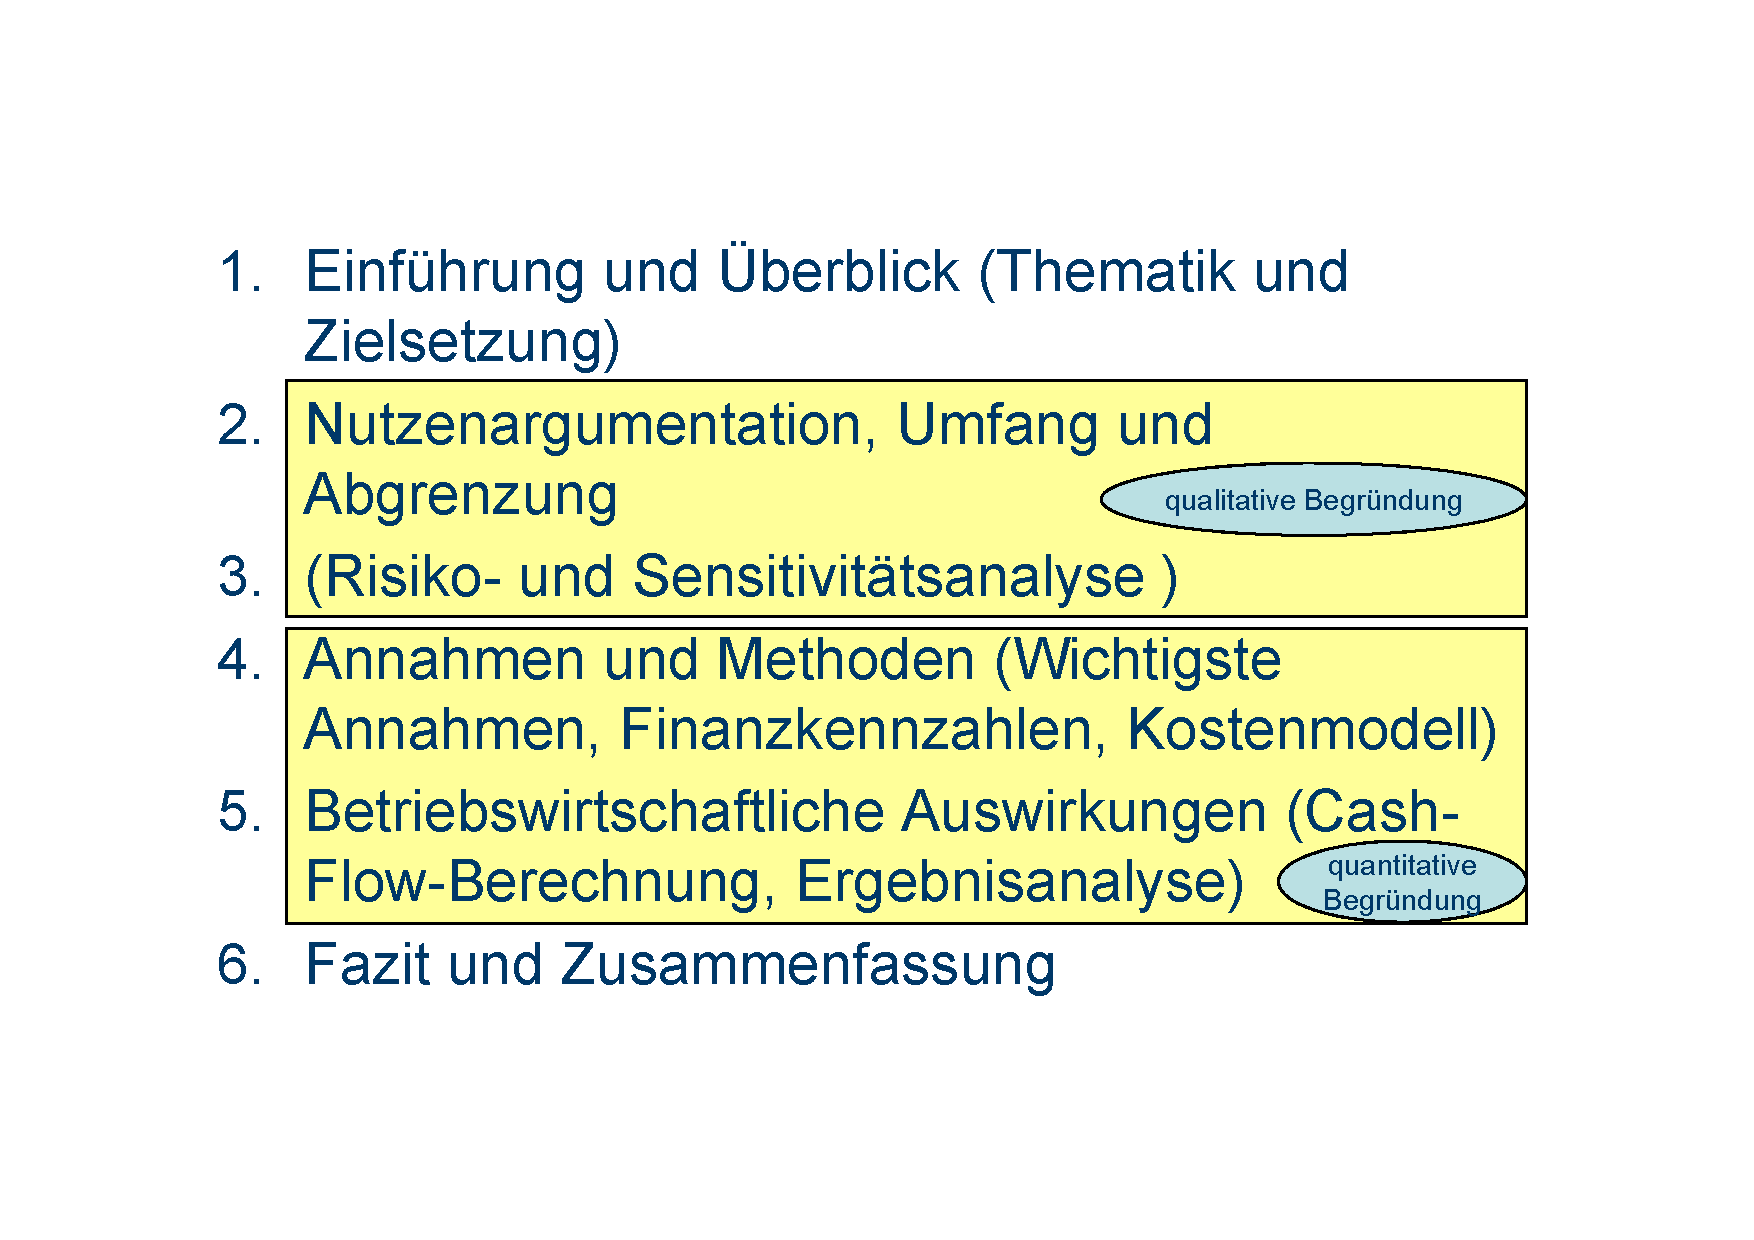
\includegraphics[width=0.7\linewidth]{fig/gliederung-business-case}
\caption{Typische Gliederung eines Business Cases}
\label{fig:gliederung-business-case}
\end{figure}


\section{Sie können die Hauptkostenarten des Total Cost of Ownership (TCO) für IT-Systeme angeben und erläutern.}

Die wichtigsten Kosten eines IT-Systems sind:
\begin{enumerate}
	\item Interne Personalkosten
	\item Externe Kosten (Personal und Dienstleistungen)
	\item Infrastrukturkosten (Räume, Rechner, Computernetzwerke)
	\item Software- resp. Lizenzkosten
\end{enumerate}
Bei den externen Personalkosten geht Geld aus der Firma raus deshalb werden externe und interne Personalkosten unterschieden.

\section{Sie können die Hauptnutzenarten für IT-Systeme angeben und erläutern.}

Der Nutzen eines IT-Systems lassen sich immer auf diese drei Arten herunterbrechen:
\begin{enumerate}
	\item Vorgaben (z. B. gesetzliche Bestimmungen) erfüllen
	\item Kostenersparnis
    \item Zusätzliche/höhere Einnahmen
\end{enumerate}

\section{Die Studierenden können einen einfachen Business Case qualitativ beschreiben.}

Um einen Business Case qualitativ beschreiben zu können braucht man gute Kenntnisse der Materie. Es gibt auch einfache Beschreibungen, wenn z.B. eine gesetzliche Vorgabe erfüllt werden muss besteht der Business Case manchmal nur aus einem Satz. Ein solches Projekt kann nur oberste Priorität haben.
Wenn eine neue Geschäftsidee umgesetzt werden soll, kann der quantitative Teil eines Business Case entfallen. Meist fehlt noch die Erfahrung in diesem neuen Umfeld und man geht das Risiko bewusst in ein, um neues Geschäftspotenzial zu nutzen.

\section{Die Studierenden können einen einfachen Business Case quantitativ beschreiben, d. h. durchrechnen.}

Bei der quantitativen Seite braucht man noch tieferes Wissen der betroffenen Gebiete, um ein realistisches Budget zu erstellen. Eine Methode zur Berechnung von Kosten und Nutzen ist die Kapitalwertmethode. Bei der Kapitalwertmethode werden alle zukünftigen Erträge (Cash Flow) auf das Jahr der Investition zurückgerechnet und mit der Investition verglichen. Die zurückgerechneten Cash Flows werden auch \emph{Net Present Value} gennant und werden nach folgender Formel berechnet: $NVP=\frac{CF}{(1+i)^n}$. Abbildung \ref{fig:kapitalwertmethode} zeigt ein Beispiel wie geprüft werden kann ob sich eine Investition lohnt.

\begin{figure}
\centering

\includegraphics[width=\linewidth]{fig/kapitalwertmethode}
\caption{Beispiel Kapitalwertmethode}
\label{fig:kapitalwertmethode}
\end{figure}
